\documentclass[11pt,letterpaper]{article}

\usepackage[T1]{fontenc}
\usepackage{lmodern}
\usepackage{microtype}
\usepackage[margin=1in]{geometry}
\linespread{1.0}
\setlength{\parskip}{0pt}          % conventional article: indent, no vertical gap
\setlength{\parindent}{1.5em}

\usepackage{amsmath,amssymb,amsthm}
\usepackage{graphicx}
\usepackage{xcolor}
\usepackage{tikz}
\usepackage{booktabs,tabularx,array,longtable}
\newcolumntype{L}[1]{>{\raggedright\arraybackslash}p{#1}}
\newcolumntype{Y}{>{\raggedright\arraybackslash}X}
\usepackage{listings}
\lstset{basicstyle=\ttfamily\footnotesize,breaklines=true,columns=fullflexible,frame=single,framesep=4pt,showstringspaces=false,captionpos=b}
\usepackage[hidelinks]{hyperref}
\usepackage{cleveref}

\newtheorem{theorem}{Theorem}[section]
\newtheorem{proposition}[theorem]{Proposition}
\newtheorem{lemma}[theorem]{Lemma}
\newtheorem{corollary}[theorem]{Corollary}
\theoremstyle{definition}
\newtheorem{definition}[theorem]{Definition}
\newtheorem{assumption}[theorem]{Assumption}
\theoremstyle{remark}
\newtheorem{remark}[theorem]{Remark}

\usetikzlibrary{arrows.meta,positioning}
\usepackage{everypage}
\definecolor{grokgray}{RGB}{110,110,110}
\AddEverypageHook{%
  \ifnum\value{page}=1
    \begin{tikzpicture}[remember picture, overlay]
      \node[rotate=90, anchor=south, font=\footnotesize\sffamily\color{grokgray}, inner sep=0pt]
        at ([xshift=30pt, yshift=0.5\paperheight]current page.south west)
        {GrokRxiv:2026.10.synthesis\quad [\,cs.DC\,]\quad 20 Oct 2026};
    \end{tikzpicture}
  \fi
}

\newcommand{\R}{\mathsf{R}}
\newcommand{\W}{\mathsf{W}}
\newcommand{\Snap}[1]{S_{#1}}
\newcommand{\Log}{\mathcal{L}}
\newcommand{\meets}{\bowtie}
\newcommand{\nmeets}{\not\bowtie}
\newcommand{\tree}{\tau}
\newcommand{\fp}{\pi_1}
\newcommand{\Later}{\mathrm{Later}}
\DeclareUrlCommand\code{\def\UrlFont{\ttfamily\small}}
\makeatletter\g@addto@macro\UrlBreaks{\do\_\do\#\do\:}\makeatother

\title{Source Code as a Transactional Abstraction\\[4pt]
  {\normalsize Foundations for Transactional Source Control, with a Serverless Realization}}
\author{Matthew Long\\
  \small The YonedaAI Collaboration, YonedaAI Research Collective\\
  \small Chicago, IL\\
  \small \texttt{matthew@yonedaai.com} \textperiodcentered\ \url{https://yonedaai.com}}
\date{October 2026}

\begin{document}
\maketitle

\begin{abstract}
Source code and source control are now transactional abstractions: a repository is a database, a change is a transaction with a read set and a write set, landing is a commit under optimistic concurrency, a version is a snapshot, and derived data, Git included, are views of a transaction log. We argue that this is the next evolution in code, the move data lakes made from files to transactional tables, and assemble its foundations from a three-part series. The transaction model gives deterministic replay, immutable snapshots and serializability relative to declared read sets; its one anomaly, write skew between members of a landing batch, is removed by a pairwise check. Derived views are consistent at a snapshot when the key of each stored partition result determines that result, and a branch's Git commit is a deterministic function of the log prefix. Composed, they let Git be built after landing without weakening the log's guarantees; a reference realization on serverless primitives measures what that buys. On one controlled deploy, the two modes that built Git trees while landing landed 4 and 385 of 1,000 concurrent writers. Appending changesets in batches landed every writer in each of six bursts of 1,000, with landing p95 of 1.2 to 3.0 s and Git commits 3.2 to 5.4 s behind at p95. Commit p95 was under 1 s in two of those runs; no sustained landing rate has been measured and no workload has exercised the write-skew check. % M204, M205, M220, M221
\end{abstract}

\section{Introduction}
\label{sec:syn:intro}

Source code and source control are now transactional abstractions. A repository is a database whose state is a map from refs to immutable objects. A change is a transaction that reads part of the source and writes another part. Landing a change is a commit under optimistic concurrency control, a version of the repository is a snapshot, and everything computed from the source, from a search index to the Git commits of a branch, is a view kept consistent with a snapshot. A series of three papers lays the foundations for that view, and its results compose into ones that no single paper states: the Git commit of a branch can be built after a change lands without weakening any guarantee of the log, and in a reference realization the landing path built on that result landed every writer in each of six bursts of 1,000. % M220, M221

We argue that this is the next evolution in code, and that data went through the same evolution first. Data lakes began as files on object stores. Concurrent writers and derived computation made a directory of files an unreliable unit of state, and the field moved to tables with a transaction log, snapshots and optimistic concurrency \cite{armbrust2020delta,icebergspec}, with partitioned computation running over those snapshots \cite{zaharia2012rdd}. Source control is now under the same pressure. Anthropic reports that its merge rate grew from about 2,500 code changes per day in May 2026 to more than 30,000 per day by September, and that source control became its largest development bottleneck \cite{anthropic2026scion}. % S-1, S-2
Scion's published design responds with server-side changesets in a write-ahead log and a ref update that is a compare-and-swap on one database row, separate from creating commits \cite{anthropic2026scion}. That is the move data made. Section~\ref{sec:syn:precedent} develops the argument and its limits.

The reason the move matters now is that the writers changed. A person clones, edits offline, pushes a finished commit and retries by hand when the branch has moved. An agent is always online, writes a few files against a head that moves while it works, and can state what it read and what it wrote. Many agents on one branch are many concurrent transactions. Git's push protocol gives them a single compare-and-swap on a ref and leaves everything else, building the commit, deciding whether the change still holds, rebasing and retesting, on the client \cite{gitprotocol}. A transactional repository moves those decisions to the server, where they can be made from recorded read and write sets.

The series supplies three foundations. Part~I gives the transaction model: a hash-chained log of ref changes, snapshots and checkpoints, backward validation of declared read and write sets, a serializability theorem, and the one place where the implemented group landing falls short of it \cite{long2026partI}. Part~II treats derived data as views over that log, maintained by partitioned jobs over immutable snapshots, and proves when incremental maintenance equals recomputation \cite{long2026partII}. Part~III builds the transaction system on cloud-portable primitives, measures it on Cloudflare as the reference realization, and models where its serialized authority saturates \cite{long2026partIII}.

The composition rests on a choice of vocabulary. Part~I states every correctness result over log entries, read sets, write sets and validation outcomes, never over Git objects. Part~II shows that the Git commit of a branch is a deterministic view of the log. Together they imply that Git objects can leave the landing path without weakening the log's guarantees, which turns the authority's critical section into a validation query and an append. Part~III's capacity model then says what limits a branch: one serial call per batch rather than one per landing. The measurements follow that chain. Landing modes that built Git trees on the landing path failed under a burst of 1,000 writers, and the mode that appends changesets in batches landed all 1,000 in every run (Section~\ref{sec:syn:evidence}). % M204, M205, M220, M221

The paper makes five contributions.
\begin{enumerate}
\item A single model of a transactional repository over six primitives, with the correspondence to transactional tables made explicit (Section~\ref{sec:syn:model}).
\item A catalogue of the series' principal theorems, each stated with its assumptions and the established result it instantiates (Section~\ref{sec:syn:results}).
\item Composition results: views consistent at a snapshot under any interleaving of landings and derivation jobs, Git semantics without Git on the landing path, batch capacity without loss of isolation, and reads served away from the authority without a change of meaning (Section~\ref{sec:syn:composition}).
\item A treatment of agents as concurrent transactions, including the condition under which the serializability guarantee extends to a task's information closure, and a map from the companion paper's equations, propositions and predictions to the series (Section~\ref{sec:syn:agents}).
\item A consolidated account of the measured evidence, with negative results, defects the analysis found, and the open problems that remain (Sections~\ref{sec:syn:evidence} and~\ref{sec:syn:open}).
\end{enumerate}

The reference implementation, YonedaRepo, is first-party work: the author designed and built it, and it is still being built. Terms such as ``authority'', ``land combiner'' and ``changeset landing'' are this project's names, not industry usage. Every claim about its code is tied to a file and commit in Appendix~\ref{app:syn:evidence} or to the Part that makes it. Every measurement comes from the Cloudflare realization; none comes from a production deployment.

\section{Precedent and pressure}
\label{sec:syn:precedent}

\subsection{Files to tables in data systems}

A data lake that stores a table as a directory of files on an object store has no atomic unit larger than one object. A writer that adds and removes several files can be seen half done, two writers can interleave, and a job that computes over the directory has no name for the state it read. Delta Lake was built to give such tables ACID transactions over cloud object stores \cite{armbrust2020delta}. Its protocol answers with a log: ``a table has a single serial history of atomic versions, which are named using contiguous, monotonically-increasing integers,'' and each log file is the unit of atomicity \cite{deltaprotocol}. A snapshot is computed by replaying the committed actions in ascending version order from a checkpoint no newer than the requested version \cite{deltaprotocol}.

The paper that introduced Delta Lake derives its isolation level from the commit step. A writer reads version $r$ and then attempts to create log record $r+1$ atomically, by put-if-absent, atomic rename or a coordination service, and because only one transaction can create each record, write transactions are serializable in increasing order of record identifiers \cite{armbrust2020delta}. Readers at a snapshot create no contention. The commit rate is bounded by the latency of the atomic step, several transactions per second on object stores, and the authors name a low-latency coordinator and batching as the remedies \cite{armbrust2020delta}. Whether a writer that retries at a later version is still correct depends on conflict checks, which the implementation states: a committing transaction fails if a concurrent commit added files that match its read predicates or removed files it read \cite{deltaconflictsrc,deltadocscc}. Iceberg reaches the same structure by an atomic swap of a metadata pointer, and its specification makes the isolation level a property of what each writer chooses to validate \cite{icebergspec}.

Computation moved with the storage. Resilient distributed datasets are read-only, partitioned collections created only by deterministic operations, and a lost partition is recomputed from its lineage \cite{zaharia2012rdd}. Over a snapshotted table, that model gives derived results a precise meaning: a result describes one version, and recomputing it from that version reproduces it.

\subsection{Pressure on source control}

Git already has immutable, content-addressed objects \cite{gitobjects}. What it lacks is a transaction around a change: its atomic step is the compare-and-swap of a ref update. A push sends, for each ref, the old and new object identifiers, and the server updates the ref only if it still holds the old value \cite{gitprotocol}. Everything before that compare-and-swap happens on the client, and when the swap fails, all of it is stale. The cost of a lost race is a fetch, a rebuild, a retest and a retry, paid in full even when the competing change touched unrelated files (Part~I, Section~2).

Agents raise both inputs to that cost. They multiply the number of concurrent writers on a branch, and they multiply derived work: checks on every candidate, search and symbol tables at every head, plans over symbol-level read and write sets. The Scion post reports a main-branch history of almost 100~GB and on the order of 25 million CI checkouts per day at one company \cite{anthropic2026scion}. % S-3, S-5
These are one organization's reported figures, used here as motivation and not as measurements of anything this series built.

\subsection{The same move in Scion's published design}

We know Scion only from its published description \cite{anthropic2026scion}. Its changesets are created on the server as entries in a write-ahead log, each listing the files changed against its first parent. A ref moves by a compare-and-swap on a single Spanner row that is not involved in creating or fetching changesets. Derived data such as blame and path history are defined recursively over a changeset's parents and computed by one generic mechanism. Read traffic passes through tiers that hold no long-lived state. Each element has a counterpart in the transactional-table design: changesets are log records, the ref row is the atomic step, derived data are views with lineage, and the tiers serve immutable objects. Scion's design does not need Git trees to land a change, and it describes itself as not a general Git replacement \cite{anthropic2026scion}.

\subsection{Scope of the argument}

Precedent constrains structure, not cost. The data-system precedent predicts that a repository under many concurrent writers will be organized as a log of atomic changes over immutable objects, with snapshot reads, validation at commit, and derived data defined per snapshot. It does not predict how fast such a system lands changes, and it does not show that the structure is necessary.

Three differences keep the analogy from being an identity, and the series treats each formally. The state of a repository is a map of refs, not a set of files, so a checkpoint is a ref map (Part~I, Section~5.4). Two writers of one file can often both succeed through a three-way merge, which has no counterpart in a table, so the model is not snapshot isolation at file granularity (Part~I, Section~6.3). And read sets are declared by the writer rather than observed by an engine, so serializability holds relative to what is declared (Part~I, Theorem~6.4). The evidence of Parts I to III supports the thesis by showing that the structure carries over with proofs, that it can be realized on generic cloud primitives, and that its measured costs fall where the theory places them. It does not show production behavior or scale beyond the bursts that were measured.

\section{A model of a transactional repository}
\label{sec:syn:model}

\subsection{Primitives}

The architecture needs six primitives, and only their contracts enter the theorems (Part~III, Section~3). Table~\ref{tab:syn:primitives} lists them with the product that realizes each in the reference implementation. A Cloudflare product is named only where the text describes that realization or its measurements. Scion's ref update, a compare-and-swap on one Spanner row \cite{anthropic2026scion,corbett2012spanner}, shows that the serialized-authority primitive is available on another cloud.

\begin{table}[t]
\centering
\small
\caption{The primitives of the architecture and their reference realization. Part~III, Table~1 adds the binding limit of each product and another documented realization.}
\label{tab:syn:primitives}
\begin{tabularx}{\textwidth}{@{}L{3.0cm}YL{3.6cm}@{}}
\toprule
Primitive & Contract the design needs & Reference realization \\
\midrule
Object store & Immutable, content-addressed puts and gets & R2, with Artifacts for Git objects \\
Serialized authority & Durable state per key, with linearizable compare-and-set on refs and log append & One Durable Object with SQLite per repository \\
Durable queue and workflow & At-least-once delivery with retries & Queues and Workflows \\
Stateless compute & Request handlers and map tasks & Workers \\
Container compute & Checks and heavy builds & Containers \\
Git projection & Serves the Git protocol from the log, optionally & Artifacts \\
\bottomrule
\end{tabularx}
\end{table}

The one property of the execution platform that the proofs use is that the authority's commands behave as if executed one at a time, each committing all of its writes or none, with no network input or output inside a command (Part~I, Assumption~4.14). Under it the authority is a state machine whose deterministic commands execute atomically with respect to one another \cite{schneider1990}, and it meets the contract that Delta's protocol states for catalog-managed tables: a catalog ``must not ratify version $v$ until it has ratified version $v-1$, and it must ratify version $v$ at most once'' \cite{deltaprotocol}. A Durable Object provides the property because it runs one request at a time and its synchronous SQLite transactions are all-or-nothing \cite{cfdoconcepts,cfdosqlite}. Any store with serializable transactions over the ref row and the log tail would provide it as well.

\subsection{State, transactions and versions}

We use Part~I's notation throughout. An object store $O$ maps 160-bit identifiers to typed bytes and only grows (Part~I, Definition~4.1). A log $\Log=(e_1,\dots,e_n)$ is a sequence of entries, each recording a version $v$, a base version $b<v$, a ref $r$, its old and new values, the touched paths $\W_v$, the declared read set $\R_v$ and a chain digest (Part~I, Definitions~4.8 to~4.10). The snapshot $\Snap{v}$ is the ref map obtained by replaying $e_1,\dots,e_v$ (Part~I, Definition~4.11), and the branch state $\sigma_v(r)$ is the tree obtained by applying, in log order, the effective changes of the entries that name $r$ (Part~I, Definition~8.1).

\begin{definition}[Transactional repository]
\label{def:syn:repo}
A \emph{transactional repository} is a tuple $(O,\Log,A,\mathcal{V})$ of an object store, a log, a serialized authority $A$ that alone appends to $\Log$ and satisfies Part~I, Assumption~4.14, and a family $\mathcal{V}$ of views. A \emph{change} on ref $r$ is $\chi=(r,b,\R,\W,\Phi)$: a base version, a declared read set of accesses at path or symbol granularity (Part~I, Definitions~4.4 and~4.6), a write set $\W$ of file paths, which the authority may refine to symbols, and a map $\Phi$ from each path of $\W$ to its new content or its deletion. \emph{Landing} $\chi$ is one command of $A$ that validates $\chi$ against the later entries $\Later(\chi)=(e_u)_{b<u\le n,\ r_u=r}$ and either refuses it or appends one entry (Part~I, Definitions~4.15 and~4.16). A \emph{view} $V\in\mathcal{V}$ assigns to each version $v$ and ref $r$ a value $V_v(r)$ that is a function of $e_1,\dots,e_v$.
\end{definition}

Validation has four outcomes (Part~I, Definition~4.15). It returns Conflict when some later entry is opaque or has a refined write that overlaps $\R$; otherwise FastForward when no later entry exists, Rebase when $\W$ meets no later entry's writes, and Merge, with the overlapping paths, when it does. The definition packages objects that Part~I owns; it adds the view family so that Git, search and checks can be discussed as one kind of object.

Table~\ref{tab:syn:correspondence} sets the model beside the transactional table. The correspondence is close enough that Part~I's main arguments are instances of Delta's, and it breaks in the rows marked by a difference in the third column.

\begin{table}[t]
\centering
\small
\caption{Transactional tables and transactional repositories. The table column follows the Delta Lake paper, protocol and implementation and the resilient distributed datasets paper; the repository column gives the result or definition of the series that plays the same role.}
\label{tab:syn:correspondence}
\begin{tabularx}{\textwidth}{@{}L{2.4cm}YY@{}}
\toprule
Concept & Transactional table & Transactional repository \\
\midrule
Unit of state & A set of data files per table & A map from refs to commits per repository (Part~I, Definition~4.11) \\
Transaction & A set of actions committed as one log record & A change with declared reads, writes and new content (Definition~\ref{def:syn:repo}) \\
Atomic step & Put-if-absent, atomic rename or a catalog that ratifies each version once & One command of the serialized authority (Part~I, Assumption~4.14) \\
Version and snapshot & Contiguous record numbers, with state replayed from a checkpoint & Contiguous log versions, with ref maps replayed from a checkpoint (Part~I, Theorem~5.1) \\
Read set & Predicates and files recorded by the engine & Accesses declared by the writer, at path or symbol granularity (Part~I, Definition~4.6) \\
Overlapping writes & A conflict, for example two deletions of one file & A three-way merge when the line merge is clean (Part~I, Proposition~6.5) \\
Isolation of writes & Serializable, or the default WriteSerializable & Serializable relative to declared reads for histories without a line merge (Part~I, Theorem~6.4) \\
Time travel & By version or by timestamp & By version or by commit identifier only \\
Retention & Removed files kept for a period, by default seven days & Hidden refs released only when safe (Part~II, Proposition~12.1) \\
Derived data & Partitions recomputed from lineage & Views keyed by content, consistent at a snapshot (Part~II, Theorem~5.3) \\
Publishing & Ratified commits published to the log directory & Git commits projected from the log (Part~II, Lemma~13.2) \\
Commit rate & Bounded by the latency of the atomic step & Bounded by the authority's service time per batch (Part~III, Proposition~6.11) \\
\bottomrule
\end{tabularx}
\end{table}

Validation is closest to Delta's Serializable level, under which reads and writes behave as if executed one by one, with the difference that the writer supplies the read predicates \cite{deltaisolationsrc}. It is not the default WriteSerializable level, which orders only writes and lets an update commit past a concurrent insert it should have read \cite{deltaisolationsrc}. The authority never reorders: the serial order is the log order, and a landing whose declared reads meet a later write is refused (Part~I, Section~5.4).

\subsection{Views}

A view is anything computed from a version: a search index, a symbol table, the blame of a file, the result of a check, the Git commit of a branch. Part~II makes the class precise. A content-local kind $\delta$ has a map function $f_\delta$ from a partition of a commit's tree to a segment and a reduce $\rho_\delta$ from the prefixed segments to a value, so that its value $D_\delta(c)$ depends only on $\tree(c)$ (Part~II, Definitions~3.2 and~4.2). A system maintains the view incrementally when it answers from stored segments, filed under keys, and the maintained view is consistent at the snapshot when its answer equals $D_\delta(c)$. A key function $\kappa$ is \emph{sufficient} for $f$ when equal keys imply equal segments (Part~II, Definition~5.1). History-dependent kinds, such as blame and path history, take the commit identifier as a sufficient key (Part~II, Corollary~5.9).

The Git commit of a branch is a view of the same kind. Under changeset landing, the projection $\Pi$ maps each log prefix and ref to a Git commit whose tree is $\sigma_v(r)$ and whose first parent is the projection of the previous prefix (Part~I, Definition~8.1 and Assumption~8.2; Part~II, Definition~13.1). It is computed after the landing returns, by a projector that reads the log.

\subsection{Cost}

The cost model is stated over the primitives' service times, with the Cloudflare measurements as one instantiation (Part~III, Section~6). A serialization point serves one operation at a time for a given key, with service time $s$; a batch point serves $k$ operations in one service of time $T(k)$ (Part~III, Definition~3.1). For $N$ agents with think time $Z$, unloaded cycle time $R_0$ and largest demand $D_{\max}$ at any serialization point, throughput $X(N)$ and cycle time $R(N)$ obey the asymptotic bounds of operational analysis \cite{denning1978operational,lazowska1984qsp}. The authority is the serialization point that every landing visits, and the land combiner or batched submission is the batch point in front of it.

\section{Principal results}
\label{sec:syn:results}

The guarantees of a transactional repository are instances of established results in concurrency control, view maintenance and queueing (Table~\ref{tab:syn:results}). Serial validation and the serializability theorem give the log its isolation, deep constructive traces and canonical serialization make views and Git projections functions of the log, and bottleneck analysis bounds what one branch can land. Each result below is proved in the Part named in its heading, and each carries the assumptions under which it holds.

\begin{table}[t]
\centering
\small
\caption{Principal results of the series. Each proof in the Parts shows that the system meets the hypotheses of the established result and names the hypotheses that differ.}
\label{tab:syn:results}
\begin{tabularx}{\textwidth}{@{}L{4.3cm}L{3.3cm}Y@{}}
\toprule
Result & Where proved & Established result it instantiates \\
\midrule
Replay determinism & Part~I, Theorem~5.1 & State-machine replication \cite{schneider1990} and Delta's action reconciliation \cite{deltaprotocol} \\
Snapshot immutability & Part~I, Theorem~5.6 & Queries of the multiversion mixed method \cite{bhg1987} \\
Refs advance along first parents, with no lost update & Part~I, Theorem~5.4 and Corollary~5.5 & Phenomenon P4 excluded on the ref item \cite{berenson1995critique} \\
Serializability relative to declared reads & Part~I, Theorem~6.4 & Serial validation \cite{kung1981occ} and the serializability theorem \cite{bhg1987} \\
Independence is order-insensitive landing without merge & Part~I, Theorem~6.7 & No conflicting operations, so both serial orders are equivalent \cite{bhg1987} \\
Batch write skew and serializable batches & Part~I, Theorem~7.3 and Proposition~7.4 & Phenomenon G2-item \cite{adya1999thesis}, write skew A5B \cite{berenson1995critique}, and the dangerous-structure theorem \cite{fekete2005serializable} \\
Carry-over to changeset landing & Part~I, Proposition~8.3 & The results above, restated over log entries \\
Incremental correctness & Part~II, Theorem~5.3 & Deep constructive traces \cite{mokhov2018build}, deterministic re-execution \cite{dean2004mapreduce} and lineage \cite{zaharia2012rdd} \\
Work bound and parent recursion & Part~II, Propositions~5.6 and~5.8 & Incremental linear operators \cite{budiu2023dbsp} \\
Determinism of the Git projection & Part~II, Lemma~13.2 & Canonical Git serialization \cite{gitobjects} \\
Asymptotic bounds and batch capacity & Part~III, Propositions~6.8 and~6.11 & Bottleneck analysis \cite{denning1978operational} and group commit \cite{dewitt1984main} \\
\bottomrule
\end{tabularx}
\end{table}

\subsection{The log}

\begin{theorem}[Replay and snapshots; Part~I, Theorems~5.1 and~5.6]
\label{thm:syn:log}
Let $\Log$ be well formed with current version $n$ (Part~I, Definition~4.10). Replaying $e_{u+1},\dots,e_v$ from the true checkpoint at $u\le v\le n$ returns $\Snap{v}$ and the chain digest $h_v$. For every later log $\Log'$ and every $u\le n$, the snapshot at $u$ computed from $\Log'$ equals the snapshot at $u$ computed from $\Log$, and every object reachable from it is unchanged if present.
\end{theorem}

The theorem has a stated limit. A checkpoint is accepted when its digest matches the log, and the digest binds it to a position but not to its ref map, so a checkpoint whose map was altered with its digest kept is detected only when the altered ref is touched again (Part~I, Theorem~5.1, second part). Delta specifies the remedy, a version checksum compared with the replayed state \cite{deltaprotocol}; the counterpart is not implemented. Presence of objects needs its own assumption, that the store keeps every object reachable from a current ref (Part~I, Assumption~5.7), and Part~II proves that the platform's release of hidden refs preserves it (Part~II, Proposition~12.1).

In the implementation at \code{cfa4845}, no code path appends a ref move or a ref deletion, every append keeps the head as first parent or creates the ref, and therefore refs advance only along first-parent chains and every landed commit stays an ancestor of its branch (Part~I, Lemma~5.3, Theorem~5.4 and Corollary~5.5). A read pinned at a version is a pure function of that version and takes no lock.

\subsection{Isolation}

\begin{theorem}[Serializability relative to declared reads; Part~I, Theorem~6.4]
\label{thm:syn:ser}
Let every entry naming $r$ above a version $v_0$ land a single commit with base at least $v_0$, directly or through a platform merge whose parents are the previous head and that commit, and not as part of a batch. Assume the serialized authority (Part~I, Assumption~4.14), a consistent base, $\fp(c)=\Snap{b}(r)$ with the writer's reads taken from $\tree(\fp(c))$ (Assumption~6.1), and sound refinement of write sets to symbols (Assumption~6.2). Then for every landing, the contents of its declared read set are the same at its base and immediately before its entry. If every landing was validated as FastForward or Rebase, the history of $r$ is conflict-serializable in log order.
\end{theorem}

Part~I proves the theorem in two steps. A landing is the end step of Kung and Robinson's serial validation, with start number $b$, finish number $n$ and the authority's command as the critical section \cite{kung1981occ}. In the serialization graph over declared locations, write-write and write-read edges point forward in log order by construction, and a backward read-write edge is exactly a stale declared read, which validation refuses; the graph is acyclic and the serializability theorem applies \cite{bhg1987}.

Two boundaries matter for agents. The guarantee is relative to declared reads: a change that reads two files and declares neither can land beside a change that wrote the other, which is write skew of shape A5B (Part~I, Example~6.6). And a Merge outcome lets two writers of one path both commit through a line-level merge, which is outside the read-write model; Part~I describes it without a serializability claim, because no theorem makes clean \texttt{diff3} merges commute \cite{khanna2007diff3}. For both reasons the system is not snapshot isolation at file granularity (Part~I, Section~6.3).

\begin{theorem}[Independence; Part~I, Theorem~6.7]
\label{thm:syn:eq1}
Let changes $c_i$ and $c_j$ share a base on ref $r$, with read and write sets at path granularity, and let nothing else land on $r$ in between. They satisfy
\begin{equation}
\W_i\nmeets(\R_j\cup\W_j)\quad\text{and}\quad\W_j\nmeets(\R_i\cup\W_i)
\label{eq:syn:independent}
\end{equation}
if and only if, in both landing orders, the second to land is validated as Rebase.
\end{theorem}

Condition~\eqref{eq:syn:independent} is Eq.~1 of the companion paper \cite{long2026inversion}, with set intersection replaced by overlap in the location tree so that a directory and a file inside it meet. The theorem gives the condition an exact operational meaning. Independence is a scheduling rule, evaluated before work runs and two-sided; validation is a safety rule, evaluated at landing against what landed and one-sided. A scheduler that ignores the condition stays safe, because validation still refuses stale reads, but it wastes the work of whichever item loses (Part~I, Section~6.4). Coarsening any access to an ancestor, a symbol to its file or a file to its directory, keeps every Conflict and Merge and can only cost concurrency (Part~I, Proposition~6.10).

\subsection{Batches}

Group landing amortizes the construction of a merge against the moving head, in the manner of group commit \cite{dewitt1984main}. Part~I proves that the combiner preserves the single-writer property of the append, whatever the state of its lease (Part~I, Theorem~7.2), and then finds its anomaly.

\begin{theorem}[Batch write skew and its repair; Part~I, Theorem~7.3 and Proposition~7.4]
\label{thm:syn:batch}
At commit \code{cfa4845}, there are histories in which the combiner lands two commits $c_a,c_b$ in one entry with $\R_a\meets\W_b$ and $\R_b\meets\W_a$, so that no serial order lets each read its declared set from the state the other leaves. If batch verification also requires, for the accepted members $c_1,\dots,c_k$ in ticket order, that $(\R_j\cup\W(c_j))\nmeets\W(c_i)$ for all $i<j$, then the batch produces the same branch state as landing the members one at a time in ticket order, and the history is conflict-serializable when every member validated as Rebase or FastForward.
\end{theorem}

The pair is a cycle of two anti-dependency edges in Adya's direct serialization graph, phenomenon G2-item \cite{adya1999thesis}, and Fekete and colleagues show that every non-serializable snapshot-isolation history contains such a structure \cite{fekete2005serializable}. Validating each member against the committed log but not against the other members is certification in the style of snapshot isolation, and this is its expected failure. The rule is sufficient, not necessary: a certifier that accepts any batch whose serialization graph is acyclic accepts strictly more \cite{bhg1987}.

Part~I then restates the model for changeset landing, in which a landing carries a base, a read set and file changes, is validated by path overlap against the log since its base, and is appended without building Git objects. Replay, immutability and serializability hold unchanged over log entries; the consistent-base assumption holds by construction because a changeset has no parent that could disagree with its base; and the first-parent and no-lost-update properties move from the ref table to the projected Git commits (Part~I, Proposition~8.3).

\subsection{Views}

\begin{theorem}[View consistency; Part~II, Theorem~5.3 and Propositions~5.4 and~5.6]
\label{thm:syn:views}
Let $\kappa$ be sufficient for $f_\delta$, let $f_\delta$ be deterministic, let every put at a key write $f_\delta$ of some partition with that key, and let gets return either nothing or a value previously put in full (Part~II, Assumption~5.2). Then every incremental evaluation at every commit $c$, under any interleaving of evaluators over any commits, returns $D_\delta(c)$. If $\kappa$ is not sufficient, some sequential order of two evaluations returns a wrong segment. With the segments of $c'$ stored and none deleted, an evaluation of $c$ runs at most one map task per partition of $c$ whose key does not occur in $c'$.
\end{theorem}

The segment store is a store of deep constructive traces: a result is filed under a hash of the task's terminal inputs, and such traces are correct only for deterministic tasks \cite{mokhov2018build}. Duplicate execution is harmless for the reason MapReduce gives \cite{dean2004mapreduce}, so last-writer-wins puts and at-least-once delivery cannot corrupt the store. The map-work bound is the incremental cost of a linear operator in DBSP, with the change taken to be the set of changed partitions \cite{budiu2023dbsp}, and content addressing reuses strictly more than recursion from parents, across reverts, cherry-picks and forks (Part~II, Proposition~5.8).

\begin{lemma}[Determinism of the Git projection; Part~II, Lemma~13.2]
\label{lem:syn:projection}
Under collision resistance of object identifiers, the projected Git commit of main at version $j$, computed by the rule of Part~II, Definition~13.1, is a function of the log prefix $e_1,\dots,e_j$. Two projectors that read the same prefix, on any replica and at any time, compute the same commit identifier.
\end{lemma}

Because the projected commit at $j$ has the projected commit at $j-1$ as first parent, the lemma discharges Part~I's Assumption~8.2, on which the first-parent and no-lost-update properties of changeset landing rest. Computing the projection at $j$ from the projection at $j-1$ rewrites only the trees on the changed paths (Part~II, Proposition~13.3).

\subsection{Capacity}

\begin{proposition}[Capacity bounds; Part~III, Propositions~6.8 and~6.11]
\label{prop:syn:capacity}
For a closed population of $N$ agents with think time $Z$ and unloaded cycle $R_0$, throughput satisfies $X(N)\le\min\{N/(R_0+Z),\,1/D_{\max}\}$, with knee $N^{*}=(R_0+Z)/D_{\max}$. A batch point whose service of $k$ operations takes $T(k)=a+bk$ with $a>0$ has capacity $k/T(k)$, which increases strictly with $k$.
\end{proposition}

The first part is Denning and Buzen's bottleneck analysis, which needs only job flow balance and visit counts and service times that do not change with load \cite{denning1978operational}. Polling breaks the second hypothesis, since a waiting landing visits the authority for as long as it waits; Part~III shows that pollers alone saturate the authority once their number exceeds the unloaded poll iteration divided by its service demand (Part~III, Corollary~6.12). The second part is the arithmetic behind group commit and behind Delta's advice to batch when the atomic step is slow \cite{dewitt1984main,armbrust2020delta}.

\section{Composition of the parts}
\label{sec:syn:composition}

The Parts were written against each other's definitions, and their results compose. Figure~\ref{fig:syn:layers} shows the dependency. Part~I's invariants, chiefly replay determinism, snapshot immutability and the first-parent discipline, are the hypotheses of Part~II's view-consistency results. Part~I's validation and Part~II's projection together determine what the authority must do inside a landing, and that is the service time Part~III's capacity model prices. The results below follow from those links and are not stated in any single Part.

\begin{figure}[t]
\centering
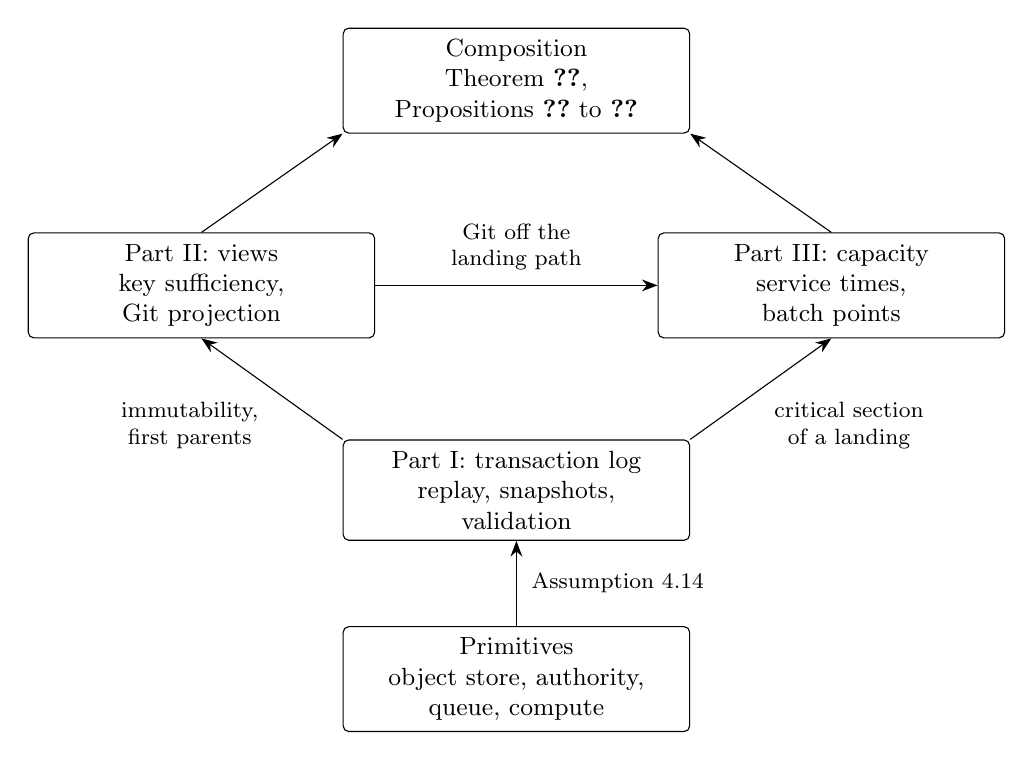
\begin{tikzpicture}[
  box/.style={draw, rounded corners=2pt, align=center, font=\small, minimum height=11mm, minimum width=4.4cm, inner sep=4pt},
  lab/.style={font=\footnotesize, align=center},
  >={Stealth[length=2mm]}]
\node[box] (prim) at (0,0) {Primitives\\object store, authority,\\queue, compute};
\node[box] (log) at (0,2.4) {Part I: transaction log\\replay, snapshots,\\validation};
\node[box] (views) at (-4.0,5.0) {Part II: views\\key sufficiency,\\Git projection};
\node[box] (cost) at (4.0,5.0) {Part III: capacity\\service times,\\batch points};
\node[box] (comp) at (0,7.6) {Composition\\Theorem~\ref{thm:syn:consistent},\\Propositions~\ref{prop:syn:offpath} to~\ref{prop:syn:reads}};
\draw[->] (prim) -- node[lab, right=2pt] {Assumption 4.14} (log);
\draw[->] (log.north west) -- node[lab, below left=2pt] {immutability,\\first parents} (views.south);
\draw[->] (log.north east) -- node[lab, below right=2pt] {critical section\\of a landing} (cost.south);
\draw[->] (views.east) -- node[lab, above=2pt] {Git off the\\landing path} (cost.west);
\draw[->] (views.north) -- (comp.south west);
\draw[->] (cost.north) -- (comp.south east);
\end{tikzpicture}
\caption{How the Parts compose. Each arrow names the result that one layer supplies to the next.}
\label{fig:syn:layers}
\end{figure}

\subsection{Consistent views under concurrent landing}

\begin{theorem}[Snapshot-consistent views]
\label{thm:syn:consistent}
Let a repository land by changesets, with the serialized authority of Part~I, Assumption~4.14 and collision-resistant object identifiers, and let the Git projection $\Pi$ of main be computed by the rule of Part~II, Definition~13.1. Let the object store keep every object reachable from a current ref (Part~I, Assumption~5.7). Let $\delta$ be a content-local kind whose key is sufficient for its map function and whose segment store satisfies Part~II, Assumption~5.2, which includes determinism of the map function. Then for every version $v$, with $r$ the main branch:
\begin{enumerate}
\item the tree $\sigma_v(r)$ and the commit $\Pi(e_1,\dots,e_v;r)$ are the same whenever and wherever they are computed, however many entries are appended later;
\item every evaluation of $\delta$ at $\Pi(e_1,\dots,e_v;r)$, under any interleaving of landings, projection jobs and derivation jobs over any commits, returns $g_\delta(\sigma_v(r))$, the value that recomputation from the snapshot gives.
\end{enumerate}
\end{theorem}

\begin{proof}
For part 1, later appends leave $e_1,\dots,e_v$ unchanged, because the authority only inserts log rows at new versions (Part~I, Theorem~5.6 and Proposition~8.3(1)); $\sigma_v(r)$ is a fold over that prefix, and $\Pi$ of the prefix is a function of the prefix by Lemma~\ref{lem:syn:projection}. For part 2, write $c=\Pi(e_1,\dots,e_v;r)$. Part~II, Theorem~5.3 holds for every interleaving of evaluators over any commits, so every evaluation at $c$ returns $D_\delta(c)$. The kind is content-local, so $D_\delta(c)=g_\delta(\tree(c))$ (Part~II, Definition~4.2), and $\tree(c)=\sigma_v(r)$ by the definition of a projection (Part~I, Definition~8.1). Landings and projection jobs enter only through part 1: they append later entries or compute projections of other prefixes, and neither changes $c$ or the segments that sufficiency ties to its partitions. Assumption~5.7 keeps the objects of $c$ readable, so every map task an evaluation needs can run.
\end{proof}

The theorem says that a view is consistent at a snapshot, not that it is fresh. A query at ``the head'' of a branch is answered at the latest projected version, which trails the log by the projection delay; on the reference realization that delay had a p95 of 3.2 to 5.4~s in the six 1,000-writer bursts at \code{fef94e7} (Section~\ref{sec:syn:batch}). % M220, M221
During the delay the log already holds the landing and every view of main is behind it.

The theorem inherits every hypothesis it composes. In the reference implementation the search key is the bare subtree identifier, while segments record full paths, so the key is not sufficient and the conclusion fails for search on renamed or duplicated directories (Part~II, Proposition~7.1). Part~II gives two repairs that restore sufficiency and proves both. Symbol tables, keyed by extension and blob identifier, satisfy the weaker form in which every reader discards the stored path (Part~II, Section~7).

\subsection{Git semantics off the landing path}

\begin{proposition}[Git semantics without Git on the landing path]
\label{prop:syn:offpath}
Assume a well-formed log, Part~I, Assumptions~4.14 and~6.2, collision-resistant object identifiers, and, as in the implementation analyzed in Part~I, Section~5.2, no command that deletes or resets the branch. A repository that lands changesets and builds the Git commits of main afterwards by the projection of Part~II, Definition~13.1, keeps the guarantees that Part~I, Proposition~8.3 lists: replay and snapshot immutability, serializability relative to declared reads, the exact meaning of Eq.~\eqref{eq:syn:independent}, the description of merged writes, and the batch results. The first-parent and no-lost-update properties hold for the projected commits. Inside the authority, a landing whose paths are disjoint from every later entry reads no file content.
\end{proposition}

\begin{proof}
Part~I, Proposition~8.3 establishes the carry-over under Assumption~8.2, and Lemma~\ref{lem:syn:projection}, which needs collision resistance, discharges Assumption~8.2. The first-parent property of projected commits follows because each entry naming main adds one first-parent step (Part~I, Proposition~8.3(5)); a command that deleted or reset the branch would end that chain, which is why the hypothesis excludes one. A disjoint landing is validated by a query of the touched paths of the entries above its base and appended; only the merge path reads the three versions of a shared file (Part~I, Section~3.6).
\end{proof}

The proposition is the theoretical reason the redesign could work. On every earlier landing path of the reference implementation, a landing that was not a fast-forward built a merge commit, with new tree objects on every changed path, before the authority appended the entry. Building Git objects there was a choice of that implementation, not a requirement of Git semantics: the requirement is that commits, branches, merges, diffs and logs keep Git's meaning, and the projection supplies them. The price is the delay before a branch's Git commit exists. The measured consequence appears in Section~\ref{sec:syn:evidence}: with Git built while landing, 4 and 385 of 1,000 concurrent landings succeeded on one deploy, and with changesets appended and Git projected afterwards, all 1,000 did. % M205, M204, M200
The comparison varies the whole landing path, so it does not separate the cost of building Git objects from the other differences between the modes, such as polling.

\subsection{Batch size and isolation}

\begin{proposition}[Batch size as a capacity parameter]
\label{prop:syn:batch}
Assume Part~I, Assumptions~4.14 and~6.2, and let a branch land changesets in batches of at most $k$ per authority command, with service time $T(k)=a+bk$, $a>0$. Let every member be validated against the log as in Part~I, Definition~4.15. Suppose further either that members are appended one at a time in ticket order, so that each is validated against a log that includes the members appended before it, or that the command defers any member whose reads or writes meet the writes of a member accepted earlier in the batch. Then every batch history is equivalent to landing its accepted members one at a time in ticket order, conflict-serializable when every member validated as FastForward or Rebase, and the branch's landing throughput is at most $k/T(k)$, which increases strictly with $k$.
\end{proposition}

\begin{proof}
In the first case each member is its own log entry, validated by Part~I, Definition~4.15 against a log that already contains the earlier members, so the batch is a sequence of single landings and Theorem~\ref{thm:syn:ser}, carried over by Part~I, Proposition~8.3(3), applies to it. In the second case the accepted members satisfy the condition of Part~I, Proposition~7.4, which applies to batches of changesets by Part~I, Proposition~8.3(6) and gives the equivalence and the serializability. The throughput bound is Part~III, Proposition~6.11 for a batch point; the authority's command is the serial step of every batch.
\end{proof}

Part~III treated the batch size as having a semantic cost as well as a latency benefit, because Part~I's Theorem~7.3 made larger batches a larger window for write skew. Under either hypothesis of the proposition that cost disappears and $k$ becomes a pure capacity parameter. The changeset path at \code{dd6c9a8} satisfies the first hypothesis by construction, and the batch path merged at \code{fef94e7} checks the second explicitly before routing each of up to 256 members (Part~I, Section~8; Appendix~\ref{app:syn:evidence}). The proposition also locates the measurable quantity: the batch call, not the landing. In the 1,000-writer run at \code{fef94e7} that kept its detail, batches held 256 landings and the batch call took 308~ms at the median and 372~ms at p95, which bounds one branch at about 690 to 830 landings per second; the measured burst-span rates of 235 to 491 per second lie below that bound (Part~III, Section~8.4). % M222, M220, M221
Those rates are averages over bursts of 2.7 to 4.3~s, not sustained rates. % M226

\subsection{Reads at a published head}

\begin{proposition}[Reads away from the authority]
\label{prop:syn:reads}
Assume collision-resistant object identifiers, and stores and caches that return either nothing or an object whose bytes hash to the requested identifier. A read of objects reachable from a commit identifier returns the same bytes from any such store or cache that holds them, and a read pinned at version $v$ returns $\Snap{v}$ or $\Pi(e_1,\dots,e_v;\mathrm{main})$ from any replica of the log prefix or of the projection, without a call to the authority.
\end{proposition}

\begin{proof}
Objects are content-addressed, so under collision resistance an identifier determines its bytes (Part~I, Definition~4.1), and a store that returns only verified objects cannot return other bytes; and reads at a commit are defined as reads of the objects reachable from it (Part~I, Definition~4.13). The snapshot at $v$ is a function of the prefix (Theorem~\ref{thm:syn:log}), and so is the projection (Lemma~\ref{lem:syn:projection}).
\end{proof}

Snapshot reads were contention-free in the model from the start: they take no lock and no landing can invalidate them. In the realization they were not, because the authority's single thread served reads, commits and landings alike. The proposition is why serving reads of main from a published head cached in stateless compute, as the realization does, leaves their meaning unchanged; what a reader gives up is recency, since the published head is a snapshot at some earlier version. Under a 1,000-writer burst, the reads served from the published head returned correct content in all 1,000 cases in each of six runs, and on an earlier revision with reads served by the authority, 540 of 1,000 succeeded and 460 were refused as overloaded. % M220, M221, M225, M227

\section{Agents as concurrent transactions}
\label{sec:syn:agents}

\subsection{Task closures as access sets}

The companion paper models a maintenance task $\tau$ by its necessary edit core $K_\tau$, its information closure $I_\tau\supseteq K_\tau$ and its required verification properties $J_\tau$ \cite{long2026inversion}. Executed as a change, the task declares a read set $\R_\tau$ and a write set $\W_\tau$. The transactional view gives the two descriptions one meaning: the closure is what the task's correctness depends on, and the declared sets are what the authority can protect. Identify each semantic unit with the location of its source text in Part~I's location tree. Say that $\R_\tau$ \emph{covers} $I_\tau$ when every location of $I_\tau$ lies in $\mathrm{sub}(x)$ for some $x\in\R_\tau$, the descendants of $x$ in the location tree (Part~I, Lemma~4.5).

\begin{proposition}[Closure coverage]
\label{prop:syn:closure}
Under the hypotheses of Theorem~\ref{thm:syn:ser}, let a task's change land on $r$ with base $b$ at version $v$, validated as FastForward, Rebase or Merge, with a declared read set that covers its information closure $I_\tau$. Then every location of $I_\tau$ has the same content at $b$ and immediately before $v$: everything the task depended on was current when it landed.
\end{proposition}

\begin{proof}
Part~1 of Part~I, Theorem~6.4 gives $\tree(\Snap{b}(r))\equiv_{\R_\tau}\tree(\Snap{v-1}(r))$, and it holds for every landing that validation did not refuse, including Merge. Agreement on $\R_\tau$ is agreement on every file and symbol location in $\bigcup_{x\in\R_\tau}\mathrm{sub}(x)$ (Part~I, Section~4.2), which contains $I_\tau$ by coverage.
\end{proof}

Coverage limits which outcomes can occur. When the task's edits lie within $I_\tau$, as edits confined to the edit core $K_\tau\subseteq I_\tau$ do, a read set that covers $I_\tau$ at path granularity covers every file the task writes; any later write to one of those files then meets $\R_\tau$, and validation returns Conflict, not Merge. Under coverage, a Merge outcome arises only when reads and refined writes are tracked at symbol granularity and a later change edited a different symbol of a file the task also edits; that is why Assumption~6.2 is among the hypotheses. The write set needs no such discipline: it is the set of touched paths, which contains every path the change edits (Part~I, Definition~4.2). Coverage of the read side is sufficient, and without it the guarantee can fail: in Part~I's Example~6.6, two changes each read two files, declare neither, and land side by side although each depended on the file the other wrote. The proposition therefore turns the companion paper's caution that independence ``is only as good as the declared sets'' \cite{long2026inversion} into a checkable condition. An agent that reports retrieval receipts, the fragments it read, can declare them as $\R_\tau$; a planner that adds referenced symbols to a chosen depth enlarges $\R_\tau$ toward $I_\tau$ (Part~II, Section~10). Two gaps remain that no declaration closes. Semantic dependencies that cross files without a lexical reference are outside any location tree, and a clean line merge can still be semantically wrong. Both are why the platform runs the policy's checks on every merged result after it lands and proposes a revert commit when one fails (Part~I, Definition~7.5), which is the companion paper's requirement that independent textual patches still receive combined acceptance.

\subsection{The companion paper in the series}

Table~\ref{tab:syn:companion} maps each element of the companion paper that the series addresses to its counterpart. The companion paper is a conceptual and mathematical framework with prospective experiments and reports no empirical study \cite{long2026inversion}; the series supplies proofs for some of its conditions and an implementation that makes two of its predictions testable.

\begin{table}[t]
\centering
\small
\caption{Elements of the companion paper and their counterparts in the series. Section and equation numbers refer to the companion paper \cite{long2026inversion}.}
\label{tab:syn:companion}
\begin{tabularx}{\textwidth}{@{}L{3.3cm}YL{3.0cm}@{}}
\toprule
Companion element & Counterpart in the series & Status \\
\midrule
Spark analogy (Section~3.2, Table~1) & Partitions are top-level subtrees, lineage is the segment key, and the only cross-partition coordination is the commit and its validation (Part~II, Table~1) & Holds for the data model and recovery, not yet for distributed execution \\
Independence (Eq.~1) & Eq.~\eqref{eq:syn:independent}, exactly the condition for order-insensitive landing without merge (Theorem~\ref{thm:syn:eq1}) & Proved \\
Critical-path bound (Eq.~2) & Plan stages meet the bound for the planner's DAG (Part~II, Theorem~10.2), and the batch call is the serial step of landing (Proposition~\ref{prop:syn:batch}) & Proved, and the batch call measured \\
Representation invariance of semantic closure (Section~5.4, Proposition~2) & Plans are unchanged under layout changes that preserve and reflect references and nesting, for symbol-level declarations (Part~II, Proposition~10.4) & Proved under that condition \\
Verification and residual risk (Section~5.5, Eqs.~15 to~17) & Checks are derived data keyed by commit, check name and policy digest (Part~II, Section~8), with post-land checks and repair commits (Part~I, Definition~7.5) & Implemented, with no coverage solver \\
Human recovery (Section~6.6, Eq.~28) & A human-only break-glass path that lands only fast-forwards and needs no check runner or queue (Appendix~\ref{app:syn:evidence}) & Implemented, with recovery time not measured \\
Dual views (Section~7.2) & The log is the single source, and Git, search and symbols are views whose regeneration is deterministic and tied to a version (Theorem~\ref{thm:syn:consistent}) & Proved for Git; the search view violates it \\
Contracts (Section~7.3) & Symbol handles bound to a commit and a digest of the symbol's bytes, with stale edits refused (Part~II, Proposition~10.6) & Implemented \\
Parallel work and conflict (Section~7.5) & Stale declared reads refused at landing, merged writes described without a serializability claim, and combined acceptance after landing (Section~\ref{sec:syn:results}) & Proved and implemented \\
\bottomrule
\end{tabularx}
\end{table}

Two rows need comment. The critical-path bound applies twice. Inside a plan, the stage of a work item is one less than the number of items on the longest chain of predecessors ending at it, so with unit durations and enough workers the stages finish in exactly the critical-path term (Part~II, Theorem~10.2(e)); the planner's fixed order makes its stage count an upper bound on the minimum, which equals the chromatic number of the conflict graph \cite{roy1967} (Part~II, Proposition~10.3). At landing, the authority's command is a mandatory serial resource that every landing passes through, and increasing the number of agents cannot remove it; batching amortizes it instead (Proposition~\ref{prop:syn:batch}). And the dual-view row is where the companion paper's warning becomes a theorem. The companion paper asks that generated views be regenerated deterministically and tied to the source revision. Lemma~\ref{lem:syn:projection} and key sufficiency are those requirements stated formally, and the search key defect is an instance of a view that drifts from its source because its key omits an input.

\subsection{Predictions and studies}

The companion paper derives predictions P1 to P9 and specifies Studies A to D. The platform makes two predictions testable. P2 says that the benefit of physical file splitting should shrink when coarse files offer equally precise symbol-level retrieval and editing; the platform provides symbol reads and edits by handle. P9 says that dependency-aware scheduling should reduce makespan and integration failures relative to file-disjoint scheduling; the platform provides declared read sets, validation and a planner. Only the following has been measured.

In the first real-model arms of Study A, with 2 to 6 tasks per arm on a deterministic synthetic codebase and one model per provider, closure recall was 1.00 in every arm and exposure precision ranged from 0.08 to 0.43. % M170, M171, M172, M173
These samples cannot test P2, and we report them only because they exist. In a two-item scripted P9 case, run once with each of two model providers with identical outcomes, file-disjoint scheduling produced a combination that failed the combined check, with 0 of 2 items accepted. Declaring read sets produced one conflict at landing and a third attempt, with 2 of 2 accepted; scheduling by the planner's stages accepted 2 of 2 in two attempts with no conflict. % M175
This is one scripted case and not a makespan measurement. Predictions P1 and P3 to P8, Studies B and C, and the fault-injection arms of Study D have no results and belong to the planned evaluation (Section~\ref{sec:syn:open}).

\section{Evidence}
\label{sec:syn:evidence}

\subsection{Setting}

All hosted measurements come from the Cloudflare realization, on an isolated deployment with its own object store, queues and Git namespace, on one account. Two clients drove the benchmarks: a live benchmark on one developer machine, whose latencies include that machine's network path, and a fan-out benchmark run from a client Worker placed in one AWS region, which can drive 1,000 writers. % M200, M220
Latencies from the two clients are not comparable as if they came from one client. Each writer commits one new file on \texttt{main} and then lands it, so the workload has no conflicting writes, no same-file merges and no declared reads. The benchmarks do not record whether the deployed tree was clean, and their outputs are uncommitted files copied into the project's evidence (Part~III, Section~11). Percentiles are over the successful requests of one run, and where several runs exist we report their range.

\subsection{Correctness evidence}

The model is tied to the code by file-and-commit tables in each Part. The platform's object identifiers reproduce identifiers computed by Git for blobs, trees and commits, and, according to the commit message that reports it, a clone of the projected repository returned the landed commit and its content and passed \texttt{git fsck} (Part~I, Section~10). % M29
The platform's three-way merge agreed with \texttt{git merge-file} on 300 of 300 randomly generated merges, both on whether the merge was clean and on its result. % M65
In a local test of the no-lost-update property, 100 of 100 concurrent writers committed and landed on one branch, a figure reported in a commit message without surviving raw output. % M60
Part~II's partition-reuse test builds 3, 1 and 0 segments for a first query, a query after a one-directory change and a query pinned at the earlier version, and checks the results (Part~II, Section~14). % test assertions, Part II Table 3

\subsection{The early commit path}

The first hosted results were negative. In the early revisions, every commit made several sequential calls to the authority and wrote its objects to the object store and the Git projection before it was acknowledged, and across four runs with 100 concurrent writers commit p95 was between 2.8~s and 3.7~s, against a design target of 1~s. % M12, M20, M30, M31
Per-phase timings attribute the miss to an unloaded commit path of 1.5 to 1.6~s at the median, of which the object-store write took 892~ms at the median in one run, and to queueing at the authority under the burst (Part~III, Section~5). % M34, M-P2.43

Taking the object-store write and the Git push off the acknowledged path brought commit p95 under 1~s. With 100 writers, 28 of 39 runs on revisions from \code{6dac346} to \code{4407515} met the target, over a full range of 437 to 2,356~ms; the four runs at \code{4407515} had 437 to 753~ms, and the two at \code{03821e0} had 638 and 805~ms. % M100, M101, M113, M114
With 1,000 writers on \code{03821e0}, commit p95 was 2,643~ms in a single run in which landings overlapped the commits. % M116

The sub-second result measures a weaker event than the early one. From \code{734c8a9} on, a commit is acknowledged once the authority or a commit shard, both durable, holds its objects; R2 and Artifacts receive their copies afterwards. That follows the architecture, in which the Git copy is a background projection, but the early revisions acknowledged a commit only after both copies existed. The benchmarks also do not record whether the deployed tree was clean.

\subsection{Landing under bursts}

Landing paths that built Git trees and merge commits inside the landing could not absorb a burst of 1,000 writers, whether waiting landings polled the authority or waited on a combiner. With polling landers at \code{a1766af}, only 20 to 306 of 1,000 landed, and in one run 980 were refused as overloaded. With the combiner at \code{03821e0}, 990 writers committed, 10 commits having failed when the bench client answered with an error, and of those 288 landed, 547 were refused as overloaded and 155 timed out. % M110, M111, M112, M116

The combiner was also slower at 100 writers. Its landing p95 was 25.7 to 30.1~s in two runs from the cloud client, against 3.65~s in the only polling run from that client, which survives in a session transcript on a revision inferred as \code{a1766af}; from the developer machine, polling at \code{4407515} gave 4.2 to 5.4~s in four runs. % M113, M114, M191, M101
Two of the combiner's alarm steps took 10.5~s and 12.5~s. The developers attribute the long steps to reading each fresh tree and blob serially through several storage layers, which is a reading of the code path, not a measurement. % M195, M196

\subsection{Controlled comparison of landing modes}

On one deploy of revision \code{dd6c9a8} on a branch, the benchmark chose the landing mode per run from one client, which isolates the effect of the landing path. Table~\ref{tab:syn:landing} gives the results with the other landing runs. At 1,000 writers, the polling mode landed 4 of 1,000, with 994 refused as overloaded, 2 failed by a storage timeout and landing p95 of 104.0~s, and the combiner landed 385 of 1,000, with 615 timeouts and landing p95 of 64.8~s. % M205, M204
The changeset mode, which appends disjoint changesets with one indexed query and builds Git commits afterwards, landed 1,000 of 1,000 with landing p95 of 18.7~s. % M200
At 100 writers the three modes had landing p95 of 2.4~s, 13.0~s and 1.2~s. % M203, M202, M201
That deploy's changeset mode still had costs that later revisions reduced: a burst-span rate of 49.7 landings per second, a Git projection delay of 17.3~s at p95, and 422 of 1,000 reads refused as overloaded. % M200

\begin{table}[t]
\centering
\small
\caption{Hosted landing results on one repository. Latencies are client-side p95 over successful requests, in seconds; entries with a range cover the runs listed. Clients: D is the developer machine and C the cloud client Worker.}
\label{tab:syn:landing}
\begin{tabularx}{\textwidth}{@{}L{1.6cm}L{4.0cm}lrrY@{}}
\toprule
Revision & Landing path & Client & Writers & Landing p95 (s) & Landed \\
\midrule
\code{4407515} & Polling, Git built & D & 100 & 4.2 to 5.4 & 100 of 100 in 4 runs \\ % M101
\code{03821e0} & Combiner, Git built & C & 100 & 25.7 to 30.1 & 100 of 100 in 2 runs \\ % M113, M114
\code{a1766af} & Polling, Git built & C & 1,000 & 24.0 to 63.1 & 20 to 306 of 1,000 in 3 runs \\ % M110, M111, M112
\code{03821e0} & Combiner, Git built & C & 1,000 & 105.5 & 288 of 990 that committed, in 1 run \\ % M116
\midrule
\code{dd6c9a8} & Polling, Git built & C & 1,000 & 104.0 & 4 of 1,000 \\ % M205
\code{dd6c9a8} & Combiner, Git built & C & 1,000 & 64.8 & 385 of 1,000 \\ % M204
\code{dd6c9a8} & Changesets & C & 1,000 & 18.7 & 1,000 of 1,000 \\ % M200
\midrule
\code{fef94e7} & Batched changesets, one token per writer & C & 1,000 & 1.21 to 1.87 & 1,000 of 1,000 in 3 runs \\ % M220
\code{fef94e7} & Batched changesets, one shared login & C & 1,000 & 2.17 to 3.03 & 1,000 of 1,000 in 3 runs \\ % M221
\code{fef94e7} & Batched changesets & C & 100 & 0.57 to 0.96 & 100 of 100 in 2 runs \\ % M224
\bottomrule
\end{tabularx}
\end{table}

\subsection{Batched landing}
\label{sec:syn:batch}

The landing redesign is merged into the development branch at \code{fef94e7}. It submits every waiting landing on a branch to the authority in one call of up to 256 landings, appends path-disjoint landings as changesets, queues landings on the same files for the merge path, defers a member whose reads or writes meet an earlier member's writes, records commits in 64 commit shards, and serves reads of main from the published head. % code constants, Appendix A rows 11-12
 In each of six 1,000-writer runs on one deploy of that revision, all 1,000 changes landed, no commit or landing was refused as overloaded, and all 1,000 reads returned the correct content. % M220, M221, M225

The results depend on whether each writer has its own token or all writers share one login. With separate tokens, commit p95 was 714 to 1,673~ms, under 1~s in two of three runs, and landing p95 was 1.21 to 1.87~s. With one shared login, commit p95 was 1,140 to 1,614~ms, missing 1~s in all three runs, and landing p95 was 2.17 to 3.03~s. % M220, M221
At 100 writers the two runs had commit p95 of 263 and 328~ms and landing p95 of 956 and 568~ms, which meets the developers' 100-writer target of 100 of 100 landed with landing p95 of at most 2~s. % M224, M198
The Git commit of main arrived 3.2 to 5.4~s after landing at p95 at 1,000 writers, down from 17.3~s on the earlier deploy. % M220, M221, M200
The burst-span landing rate was 404 to 491 per second with separate tokens and 235 to 284 with one login, over bursts that lasted 2.7~s and 4.3~s end to end in the runs that recorded it. % M220, M221, M226
Only the third run of each set kept its full output; the first two survive as summary lines printed from their output before it was overwritten. % M220, M221

These results confirm the direction of Proposition~\ref{prop:syn:offpath} on one deploy and one client. They do not establish a sustained landing rate, which no run has measured, and they do not exercise the within-batch write-skew check, because every writer writes its own file and declares no reads.

\subsection{Defects found by the analysis}

The proofs found three gaps between the implementation and the model, and the analysis of derived data found a fourth.

Batch write skew was found by proof, not by test. At \code{cfa4845} and \code{03821e0}, the combiner validates batch members against the log and not against each other, so two members that each read what the other wrote can land in one entry (Theorem~\ref{thm:syn:batch}). Revision \code{c4c8f47} added the check of Part~I, Proposition~7.4 to the combiner and to batch verification, and the batch path merged at \code{fef94e7} calls it for every member and defers a member that fails (Appendix~\ref{app:syn:evidence}). The check has not been exercised by any hosted run.

Writer-supplied parents were not checked against the base version, which leaves exposed a base strictly between the parent's version and the head (Part~I, Section~6.1). The changeset route checks it, because a commit takes that route only if its single parent is the projected head at its base (Part~I, Section~8), and the route is on the development branch from \code{fef94e7}. Checkpoints are trusted on their digest alone, and that gap is open.

The search view is not consistent at every snapshot. Its key is the bare subtree identifier, while its segments record full paths, so a renamed directory reuses a segment that names the old paths, and two identical top-level directories share one segment that names only one of them (Part~II, Proposition~7.1). The consequences reach access control: grant filtering uses the stored paths, so a caller can receive matches from files under a directory its grant does not cover (Part~II, Section~7). A test executed against the crates at \code{cfa4845} confirms the key collision; the effects on search responses were traced through the adapter and not run (Part~II, Appendix~B). Part~II proves two repairs, of which relative paths with a prefixing reduce keeps reuse across renames and forks.

\subsection{The model against the measurements}

Part~III's capacity model is the one place where the series projects beyond what was measured, and every projected figure below is labelled as such. Using parameters taken from local and per-phase timings rather than from the tails themselves, the burst predictor reproduces the commit p95 of the four early 100-writer runs within 18 percent (Part~III, Section~7). % M10, M20, M30, M31
The model projected that configurations whose waiting landings poll the single-threaded authority collapse first, and on the controlled deploy the polling mode did fail first; it was wrong about the form of the failure, since the platform refuses requests that queue too long rather than letting waits grow (Part~III, Section~8.4). % M205
Its projected ceiling for the non-polling combiner, about 11 landings per second, bounds the measured burst rates of 7.0 and 5.9 per second at 100 and 1,000 writers (Part~III, Section~8.4). % M202, M204
The batch-capacity relation bounds the redesign's measured rates, as Proposition~\ref{prop:syn:batch} requires. The projections describe a steady state that no run reached, and none of them is a measurement.

\section{Relation to Scion}
\label{sec:syn:scion}

Scion and this series make the same structural move, and their evidence is not comparable. Scion's published design reports more than 30,000 merges per day, an average of about 0.35 per second, and no landing latency under bursts \cite{anthropic2026scion}. % S-2
The runs reported here are bursts of 100 to 1,000 landings on one branch of one repository within seconds. % M101, M220, M221
 We make no claim that the system studied here is faster or slower than Scion, and no claim about its behavior under Scion's workload.

The designs differ in three places, each with a measured consequence (Part~III, Section~10). Scion moves a ref by a compare-and-swap on one Spanner row; this architecture places every ref, the log and, in the measured revisions, commit authorization behind one authority per repository, so serialization is per repository and one hot repository is the unit of capacity. That is a choice of key for the authority, not a property of the primitive. Scion's changesets need no tree objects; the measured revisions built Git trees until changeset landing moved them into a projection. And this platform gates landing on approvals and required checks, where Scion's published design lands without a global merge lock and tests after merge. The Scion post credits Mononoke, the server of Meta's Sapling, with pioneering many of its techniques, in particular the Bonsai data model of flat file changes \cite{anthropic2026scion,mononokebonsai}.

\section{Related work}
\label{sec:syn:related}

The transactional table is the template. Delta Lake's paper gives the log, the checkpoints, the put-if-absent commit and the argument that writes are serializable in record order \cite{armbrust2020delta}; its protocol fixes the naming, the replay rule, the version checksum and the ratification contract of catalog-managed tables \cite{deltaprotocol}; and its implementation states the conflict checks and isolation levels that the paper leaves open \cite{deltaconflictsrc,deltaisolationsrc,deltadocscc}. Iceberg reaches the same guarantees by an atomic swap of a metadata pointer and makes the isolation level a property of what each writer validates \cite{icebergspec}. The series takes this structure intact and changes three things: the atomic step is a command of a serialized authority, read sets are declared at path or symbol granularity, and overlapping writes to one file are merged.

Optimistic concurrency control begins with Kung and Robinson, whose serial validation is the landing step \cite{kung1981occ}. The serializability theorem, the treatment of granularity and the certifiers come from Bernstein, Hadzilacos and Goodman \cite{bhg1987}. The isolation vocabulary is that of Berenson and colleagues \cite{berenson1995critique} and of Adya, whose graph phenomena classify the batch anomaly \cite{adya1999thesis}, and Fekete and colleagues characterize when snapshot isolation fails to be serializable \cite{fekete2005serializable}. What source control adds is the write-write case: a change to a file is a patch, and two patches to different regions can both apply, with the caveat that the intuition behind clean \texttt{diff3} merges is false in its obvious formulations \cite{khanna2007diff3}.

Incremental view maintenance updates a materialized view after its base data change, on the heuristic that only part of a view changes \cite{gupta1995maintenance}, and DBSP turns queries into incremental programs whose linear parts cost in proportion to the change \cite{budiu2023dbsp}. Build systems memoize task results under hashes of their inputs and are correct only when the hash covers every input and the task is deterministic \cite{mokhov2018build}. Part~II's key sufficiency is that requirement for partitioned derived data, and the search key defect is the classic build error of a task reading an input, its own location, that its key omits. Mononoke separates core data from derived data computed afterwards and derives each changeset's value from its parents' \cite{mononokederived}; content addressing by Git tree reuses more for content-local kinds and leaves history-dependent kinds keyed by commit.

Among source-control systems, Scion is closest in intent \cite{anthropic2026scion}, Mononoke's pushrebase is the nearest precedent for landing on the server \cite{mononokepushrebase}, and Google's Piper is the long-standing example of one very large repository with a server-side source of truth \cite{potvin2016piper}. The series differs from these in keeping Git's objects and identifiers, so every exposed commit can be fetched and verified by stock Git, and in validating declared read sets rather than file overlap alone.

\section{Open problems}
\label{sec:syn:open}

The foundation leaves seven questions open, each tied to a measurement or a proof that does not yet exist.

\paragraph{Sustained landing rate.} Every 1,000-writer result is a burst of a few seconds, and its rate is an average over the burst span (Section~\ref{sec:syn:batch}). The developers' target of 1,000 of 1,000 landed at a sustained 50 per second has not been tested. % M198
Part~III plans open-loop arrivals at fixed rates from 50 to 800 landings per second for at least ten minutes each, % planned rates, Part III Section 9
 logging every batch call, so that the batch-capacity relation is tested directly and the highest rate held without refusals locates the knee (Part~III, Section~9).

\paragraph{Authority reads under a burst.} Reads survive the burst because they avoid the authority (Proposition~\ref{prop:syn:reads}). With reads served by the authority on an earlier revision, 460 of 1,000 were refused. % M227
A read that needs the authority's current state, rather than a published snapshot, still competes with commits and landings for one thread. The planned run repeats the burst with each read source and counts a refused read as a failed run.

\paragraph{Commit p95 under a shared login.} With one shared login, commit p95 missed 1~s in all three 1,000-writer runs, and the shared login's authorization phase took 381~ms at the median in the run that kept its detail. % M221, M223
Whether the shared session's checks account for the difference is untested.

\paragraph{Write skew within a batch.} The check that removes batch write skew is in the merged code and has never run on a workload that could trigger it. A workload whose writers read files that other members of the same batch write would measure how often members are deferred and what deferral costs.

\paragraph{Git delay.} Main's Git commit trails the log by 3.2 to 5.4~s at p95 under a burst. % M220, M221
No run measures the delay under sustained load, and no bound on it has been proved; Theorem~\ref{thm:syn:consistent} guarantees consistency at a snapshot, not freshness.

\paragraph{Checkpoint validation.} A checkpoint whose ref map was altered while its digest was kept is detected only when the altered ref is touched again. A digest of the ref map stored with each checkpoint and in the next entry, the counterpart of Delta's version checksum \cite{deltaprotocol}, would close the gap; it is not built and no test exercises it.

\paragraph{Planned evaluation.} Part~III's Section~9 is the planned evaluation for the whole series. Beyond the items above, it measures the authority's service time per call type by saturation, the land combiner's batch sizes and cycle times, push sizes, per-tier hit rates under cold reads, and the costs that Part~II lacks: segment build time and size, the fraction of partitions that change per landing on real repositories, and the delay from landing to a queryable segment. It also runs the companion paper's Study A and P9 at a size that can test them, with closure recall, exposure precision and cost per accepted change as metrics \cite{long2026inversion}. Each item names the outcome that would refute its expectation.

Two further limits are structural. Serializability holds per ref, like Delta's per-table limit, and nothing in the model gives atomicity across refs or repositories \cite{armbrust2020delta}. And log compaction and retention are not designed, which matters because the authority's database is bounded and a repository at Scion's merge rate would add tens of thousands of entries per day (Part~III, Section~4). % S-2

\section{Threats to validity}
\label{sec:syn:threats}

The theorems are proved about a model, and the model's correspondence with the code was established by reading the code at pinned commits, not by mechanized verification. The interleavings of landing, claiming and leasing were tested by example, not explored exhaustively, and a model-checked test of them is the strongest missing piece of correctness evidence (Part~I, Section~12).

The performance evidence comes from one account, two client locations and few runs per revision. The early group's run-to-run spread of commit p95 was 0.93~s across four runs, so no single run should be read as precise. % M12, M20, M30, M31
The deployed tree's cleanliness was never recorded, the outputs of the later runs exist only as uncommitted files, and for the \code{fef94e7} runs the bench client carried an uncommitted change that reports commits per shard. The workload is synthetic: one tiny new file per writer, with no conflicting writes and no declared reads, so it exercises the disjoint fast path and nothing else.

The acceptance point moved during the series. The sub-second commit results count a commit as accepted once a Durable Object holds its objects, the early results once the object store and the Git projection did. The two groups do not measure the same event, and the paper never compares them as if they did.

The capacity projections rest on assumptions that no run has tested at sustained saturation: uniform cost per authority call, a closed population with fixed think time, and a combiner cycle independent of batch size (Part~III, Section~11). They are labelled as projections wherever they appear.

\section{Conclusion}
\label{sec:syn:conclusion}

A repository can be run as a transactional database, and the guarantees of transactional tables carry over with proofs: deterministic replay, immutable snapshots, and landings serializable in log order relative to what they declare they read, whenever no line-level merge is needed. Derived data become views that are guaranteed consistent at a snapshot exactly when their keys determine their stored results, and Git becomes one of those views. The composition is the practical result. Because every guarantee is stated over log entries and the Git commit of a branch is a deterministic function of the log, Git objects can leave the landing path, and the authority's work per landing shrinks to a validation query and an append, batched. The measurements follow the theory on one realization: landings that built Git while landing failed under a burst of 1,000 writers, and batched changesets landed every writer in every run.

What the foundation enables is a source-control system whose correctness rests on a transaction log and whose cost can be stated per primitive before it is built on a particular cloud. It also gives the companion paper's conditions a precise meaning at landing: independence is exactly order-insensitive landing without merge, and a task's information closure is protected wherever its declared read set covers it. What remains open is quantitative and empirical: a sustained landing rate, reads that need the authority under load, commits under a shared login, the Git delay, and a workload that exercises write skew within a batch.

\begin{thebibliography}{99}
\small

\bibitem{adya1999thesis}
A.~Adya.
Weak consistency: A generalized theory and optimistic implementations for distributed transactions.
PhD thesis, Massachusetts Institute of Technology, March 1999. MIT-LCS-TR-786.
\url{https://dspace.mit.edu/handle/1721.1/149899}.

\bibitem{anthropic2026scion}
Nick G. and the source control team.
Redesigning source control at Anthropic.
Anthropic Engineering, 13 October 2026, updated 15 October 2026.
\url{https://www.anthropic.com/engineering/redesigning-source-control}.

\bibitem{armbrust2020delta}
M.~Armbrust, T.~Das, L.~Sun, B.~Yavuz, S.~Zhu, M.~Murthy, J.~Torres, H.~van Hovell, A.~Ionescu, A.~{\L}uszczak, M.~{\'S}witakowski, M.~Szafra{\'n}ski, X.~Li, T.~Ueshin, M.~Mokhtar, P.~Boncz, A.~Ghodsi, S.~Paranjpye, P.~Senster, R.~Xin, and M.~Zaharia.
Delta Lake: High-performance ACID table storage over cloud object stores.
\emph{Proceedings of the VLDB Endowment}, 13(12):3411-3424, 2020.
doi:10.14778/3415478.3415560.

\bibitem{berenson1995critique}
H.~Berenson, P.~Bernstein, J.~Gray, J.~Melton, E.~O'Neil, and P.~O'Neil.
A critique of ANSI SQL isolation levels.
In \emph{Proceedings of the 1995 ACM SIGMOD International Conference on Management of Data}, pages 1-10, 1995.
doi:10.1145/223784.223785.

\bibitem{bhg1987}
P.~A. Bernstein, V.~Hadzilacos, and N.~Goodman.
\emph{Concurrency Control and Recovery in Database Systems}.
Addison-Wesley, 1987.
\url{https://www.microsoft.com/en-us/research/people/philbe/book/}.

\bibitem{budiu2023dbsp}
M.~Budiu, T.~Chajed, F.~McSherry, L.~Ryzhyk, and V.~Tannen.
DBSP: Automatic incremental view maintenance for rich query languages.
\emph{Proceedings of the VLDB Endowment}, 16(7):1601-1614, 2023.
doi:10.14778/3587136.3587137.

\bibitem{cfdoconcepts}
Cloudflare.
What are Durable Objects?
Cloudflare Durable Objects documentation.
\url{https://developers.cloudflare.com/durable-objects/concepts/what-are-durable-objects/}.

\bibitem{cfdosqlite}
Cloudflare.
SQLite-backed Durable Object Storage.
Cloudflare Durable Objects documentation.
\url{https://developers.cloudflare.com/durable-objects/api/sqlite-storage-api/}.

\bibitem{corbett2012spanner}
J.~C. Corbett, J.~Dean, M.~Epstein, A.~Fikes, et~al.
Spanner: Google's globally-distributed database.
In \emph{10th USENIX Symposium on Operating Systems Design and Implementation (OSDI 12)}, 2012.
\url{https://www.usenix.org/conference/osdi12/technical-sessions/presentation/corbett}.

\bibitem{dean2004mapreduce}
J.~Dean and S.~Ghemawat.
MapReduce: Simplified data processing on large clusters.
In \emph{Proceedings of OSDI}, 2004.
\url{https://www.usenix.org/legacy/events/osdi04/tech/dean.html}.

\bibitem{deltaconflictsrc}
Delta Lake project.
ConflictChecker.scala, commit d99585d.
\url{https://github.com/delta-io/delta/blob/d99585d85ad94660dcd88fd798a1d5241edebc4c/spark/src/main/scala/org/apache/spark/sql/delta/ConflictChecker.scala}.

\bibitem{deltadocscc}
Delta Lake project.
Concurrency control.
\url{https://docs.delta.io/latest/concurrency-control.html}.

\bibitem{deltaisolationsrc}
Delta Lake project.
isolationLevels.scala.
\url{https://github.com/delta-io/delta/blob/master/spark/src/main/scala/org/apache/spark/sql/delta/isolationLevels.scala}.

\bibitem{deltaprotocol}
Delta Lake project.
Delta transaction log protocol (PROTOCOL.md).
\url{https://github.com/delta-io/delta/blob/master/PROTOCOL.md}.

\bibitem{denning1978operational}
P.~J. Denning and J.~P. Buzen.
The operational analysis of queueing network models.
\emph{ACM Computing Surveys}, 10(3):225-261, 1978.
doi:10.1145/356733.356735.

\bibitem{dewitt1984main}
D.~J. DeWitt, R.~H. Katz, F.~Olken, L.~D. Shapiro, M.~R. Stonebraker, and D.~Wood.
Implementation techniques for main memory database systems.
In \emph{Proceedings of the 1984 ACM SIGMOD International Conference on Management of Data}, pages 1-8, 1984.
doi:10.1145/602259.602261.

\bibitem{fekete2005serializable}
A.~Fekete, D.~Liarokapis, E.~O'Neil, P.~O'Neil, and D.~Shasha.
Making snapshot isolation serializable.
\emph{ACM Transactions on Database Systems}, 30(2):492-528, 2005.
doi:10.1145/1071610.1071615.

\bibitem{gitobjects}
S.~Chacon and B.~Straub.
Git internals: Git objects.
In \emph{Pro Git}, second edition.
\url{https://git-scm.com/book/en/v2/Git-Internals-Git-Objects}.

\bibitem{gitprotocol}
Git project.
gitprotocol-pack: How packs are transferred over-the-wire.
\url{https://git-scm.com/docs/gitprotocol-pack}.

\bibitem{gupta1995maintenance}
A.~Gupta and I.~S. Mumick.
Maintenance of materialized views: Problems, techniques, and applications.
\emph{IEEE Data Engineering Bulletin}, 18(2):3-18, 1995.
\url{http://sites.computer.org/debull/95JUN-CD.pdf}.

\bibitem{icebergspec}
Apache Iceberg project.
Iceberg table spec.
\url{https://iceberg.apache.org/spec/}.

\bibitem{khanna2007diff3}
S.~Khanna, K.~Kunal, and B.~C. Pierce.
A formal investigation of diff3.
In \emph{FSTTCS 2007: Foundations of Software Technology and Theoretical Computer Science}, Lecture Notes in Computer Science, pages 485-496. Springer, 2007.
doi:10.1007/978-3-540-77050-3\_40.

\bibitem{kung1981occ}
H.~T. Kung and J.~T. Robinson.
On optimistic methods for concurrency control.
\emph{ACM Transactions on Database Systems}, 6(2):213-226, 1981.
doi:10.1145/319566.319567.

\bibitem{lazowska1984qsp}
E.~D. Lazowska, J.~Zahorjan, G.~S. Graham, and K.~C. Sevcik.
\emph{Quantitative System Performance: Computer System Analysis Using Queueing Network Models}.
Prentice-Hall, 1984.
\url{https://homes.cs.washington.edu/~lazowska/qsp/}.

\bibitem{long2026inversion}
M.~Long and The YonedaAI Collaboration.
The inversion of software maintainability in AI-native repositories.
YonedaAI Research Collective, author's manuscript, 14 October 2026.

\bibitem{long2026partI}
M.~Long and The YonedaAI Collaboration.
A transaction log for source control.
Part I of \emph{Source Code as a Transactional Abstraction}, YonedaAI Research Collective, author's manuscript, October 2026.

\bibitem{long2026partII}
M.~Long and The YonedaAI Collaboration.
Partitioned derived data.
Part II of \emph{Source Code as a Transactional Abstraction}, YonedaAI Research Collective, author's manuscript, October 2026.

\bibitem{long2026partIII}
M.~Long and The YonedaAI Collaboration.
A cloud-portable architecture for serverless Git.
Part III of \emph{Source Code as a Transactional Abstraction}, YonedaAI Research Collective, author's manuscript, October 2026.

\bibitem{mokhov2018build}
A.~Mokhov, N.~Mitchell, and S.~Peyton Jones.
Build systems {\`a} la carte.
\emph{Proceedings of the ACM on Programming Languages}, 2(ICFP), Article 79, 2018.
doi:10.1145/3236774.

\bibitem{mononokebonsai}
Sapling project.
Mononoke: Bonsai data model.
\url{https://github.com/facebook/sapling/blob/main/eden/mononoke/docs/2.1-bonsai-data-model.md}.

\bibitem{mononokederived}
Sapling project.
Mononoke: Derived data.
\url{https://github.com/facebook/sapling/blob/main/eden/mononoke/docs/2.3-derived-data.md}.

\bibitem{mononokepushrebase}
Sapling project.
Mononoke: Pushrebase.
\url{https://github.com/facebook/sapling/blob/main/eden/mononoke/docs/4.1-pushrebase.md}.

\bibitem{potvin2016piper}
R.~Potvin and J.~Levenberg.
Why Google stores billions of lines of code in a single repository.
\emph{Communications of the ACM}, 59(7):78-87, 2016.
doi:10.1145/2854146.

\bibitem{roy1967}
B.~Roy.
Nombre chromatique et plus longs chemins d'un graphe.
\emph{Revue fran\c{c}aise d'informatique et de recherche op\'erationnelle}, 1(5):129-132, 1967.
\url{http://www.numdam.org/item/M2AN_1967__1_5_129_0/}.

\bibitem{schneider1990}
F.~B. Schneider.
Implementing fault-tolerant services using the state machine approach: A tutorial.
\emph{ACM Computing Surveys}, 22(4):299-319, 1990.
doi:10.1145/98163.98167.

\bibitem{yonedarepo}
M.~Long.
YonedaRepo source repository, branch \texttt{dev}, with the commits named in Appendix~\ref{app:syn:evidence}, 20 October 2026.
Private repository; not publicly available.

\bibitem{zaharia2012rdd}
M.~Zaharia, M.~Chowdhury, T.~Das, A.~Dave, J.~Ma, M.~McCauley, M.~J. Franklin, S.~Shenker, and I.~Stoica.
Resilient distributed datasets: A fault-tolerant abstraction for in-memory cluster computing.
In \emph{9th USENIX Symposium on Networked Systems Design and Implementation (NSDI 12)}, pages 15-28, 2012.
\url{https://www.usenix.org/conference/nsdi12/technical-sessions/presentation/zaharia}.

\end{thebibliography}

\appendix

\section{Code evidence}
\label{app:syn:evidence}

Table~\ref{tab:syn:evidence} ties each claim this paper makes about the implementation, beyond what it cites to a Part, to a file and commit in the YonedaRepo repository \cite{yonedarepo}. Commits are on the development branch unless a branch is named; \code{dd6c9a8} and \code{c4c8f47} were made on branch \code{claude/native-p95e}, which reached the development branch with the merge \code{f9d9c14}. Paths are relative to the repository root, and \code{store} abbreviates \code{backend/crates/yoneda-platform/src/repo_store}.

\begin{small}
\begin{longtable}{@{}L{0.7cm}L{3.2cm}L{4.0cm}L{1.3cm}L{4.8cm}@{}}
\caption{Claims about the implementation and the code that shows them.}\label{tab:syn:evidence}\\
\toprule
Row & Claim & File & Commit & What the code shows \\
\midrule
\endfirsthead
\toprule
Row & Claim & File & Commit & What the code shows \\
\midrule
\endhead
\bottomrule
\endfoot
1 & Validation has four outcomes & \code{backend/crates/yoneda-core/src/txlog/occ.rs} & \code{cfa4845} & The outcome type has the cases FastForward, Rebase, Merge and Conflict, and a later entry without touched paths whose kind is neither commit nor merge yields a Conflict. \\
2 & Independence is two-sided & \code{backend/crates/yoneda-core/src/txlog/access.rs} & \code{cfa4845} & \code{independent} returns true only when neither write set meets the other change's reads or writes. \\
3 & A landing appends its entry, ref, projection target, checkpoint and landing record together & \code{store/land.rs} & \code{cfa4845} & \code{append} inserts the log row, upserts the ref, sets the projection target, calls \code{maybe_checkpoint} and inserts the landings row using only SQL calls. \\
4 & The combiner checks members against the log and not against each other & \code{store/land_queue.rs} & \code{cfa4845} & \code{verify_octopus} checks the parents, the merge principal, each member's validation against the log and the changed paths, with no check between members. \\
5 & Time travel is by version or commit only & \code{store/reads.rs} & \code{cfa4845} & \code{at} accepts only a version from 0 to the current version, \code{refs_at} replays from the nearest accepted checkpoint, and no timestamp form exists. \\
6 & Human-only break-glass recovery & \code{store/break_glass.rs}, \code{store/auth.rs}, \code{backend/crates/yoneda-platform/src/repo_store.rs} & \code{cfa4845} & The module comment states that a signed-in human owner can land past failing or pending checks, revert, release a stuck lease or pause automation without a check runner or queue, and that recovery is a new commit fast-forwarded onto the head; the dispatcher requires \code{require_human_owner} for \code{repo_break_glass}, which returns \code{break_glass::refusal} to every caller that is not a signed-in human owner. \\
7 & The search key is the bare subtree identifier & \code{backend/crates/yoneda-platform/src/platform_derived.rs} & \code{cfa4845} & \code{plan} emits each directory partition with \code{"key": e.id} beside \code{"prefix": e.name}. \\
8 & Changesets are validated by the log's path index & \code{store/changesets.rs} & \code{dd6c9a8} & \code{route} sends a commit to the changeset route and tests its touched paths and read set with \code{touched_since} against entries above its base; a command lands at most \code{BATCH} = 128 members. \\
9 & The Git projection uses only the previous head, the landed commit and fields of the entry & \code{backend/crates/yoneda-platform/src/platform_project.rs} & \code{dd6c9a8} & \code{project_changesets} builds each commit from the previous head's tree and the landed commit's tree at its changed paths, with a constant author, the landing time and a message from the commit identifier and version. \\
10 & A batch member that meets earlier writes is refused & \code{store/land_queue.rs}, \code{store/merging.rs} & \code{c4c8f47} & Batch verification returns \code{WRITE_SKEW} when \code{BatchWrites::admits} finds that a member reads or writes a path an earlier accepted member wrote. \\
11 & The merged batch path defers a skewing member & \code{store/submitted.rs} & \code{fef94e7} & The submit command accepts at most 256 landings and defers a member when \code{admits} fails on its read set and touched paths; a member routed as a changeset or fast-forward is appended as a changeset entry and its writes are recorded with \code{accept}, and a member routed to the merge path is adopted and queued. \\
12 & Batch mode, reads from the published head and 64 shards are configured & \code{cloudflare/wrangler.platform.jsonc}, \code{cloudflare/worker/repo-shards.ts} & \code{fef94e7} & \code{LAND_MODE} is \code{batch} with \code{BEGIN_MODE} and \code{READ_MODE} set to \code{head}, and \code{SHARDS} is 64. \\
\end{longtable}
\end{small}

\end{document}
